% !TEX encoding = UTF-8
% !TEX TS-program = pdflatex
% !TEX root = ../../tesi.tex

\section{Analisi dei requisiti}
Ho iniziato la fase di analisi dei requisiti dalla quarta settimana di lavoro, cioè quando, come pianificato, avrei dovuto iniziare ad implementare gli \textit{smart contract} per la gestione di NFT seguendo gli standard ERC su \textit{blockchain} Ethereum. Inizialmente è avvenuto un processo di \textit{brainstorming} con gli altri componenti del gruppo e i vari \textit{tutor} di ognuno di noi per definire al meglio le funzionalità della piattaforma. In seguito ho isolato e ridotto le funzionalità ed i requisiti che avrebbe dovuto avere la libreria e lo \textit{smart contract} da implementare. Per quanto riguarda i casi d'uso, vengono utilizzati i diagrammi dei casi d'uso per facilitarne la Presentazione concettuale, mentre per i requisiti sono state utilizzate delle tabelle di tracciamento. 

\subsection{Casi d'uso}
I casi d'uso sono una tecnica utilizzata nel processo di analisi dei requisiti per effettuare in maniera esaustiva e non ambigua la raccolta dei requisiti al fine di produrre \textit{software} di qualità. \\

\noindent La classificazione dei casi d'uso ha seguito la seguente convenzione:
\begin{center}
  UC[NumeroCasoBase](.[NumeroSottoCaso])*
\end{center}
dove:
\begin{itemize}
  \item \textbf{NumeroCasoBase}: è costituito da un numero progressivo che indica il caso d'uso generico;
  \item \textbf{NumeroSottoCaso}: è costituito da un numero progressivo opzionale che indica il sotto-caso d'uso del caso
  d'uso generico.
\end{itemize}

\subsubsection{Attori primari}
Un attore primario è colui che interagisce con il sistema per un determinato scopo.
Gli attori primari che sono stati identificati sono i seguenti:

\begin{figure}[h!]
  \centering
  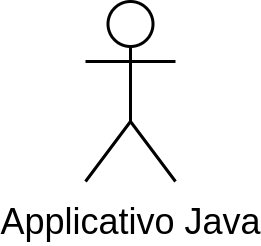
\includegraphics{capitolo3/casi-uso/attori-primari.png}
  \caption{Attori primari}
\end{figure}

\begin{itemize}
  \item \textbf{Applicativo Java}: rappresenta qualsiasi applicazione sviluppata in Java che interagisce con la libreria. Nel contesto di NFTLab, consiste nel \textit{back-end} sviluppato utilizzando il \textit{framework} Spring.
\end{itemize}

\subsubsection{Attori secondari}
Un attore secondario è un'entità estranea al sistema che supporta gli attori primari nelle loro attività. Gli attori secondari che sono stati identificati sono i seguenti:

\begin{figure}[h!]
  \centering
  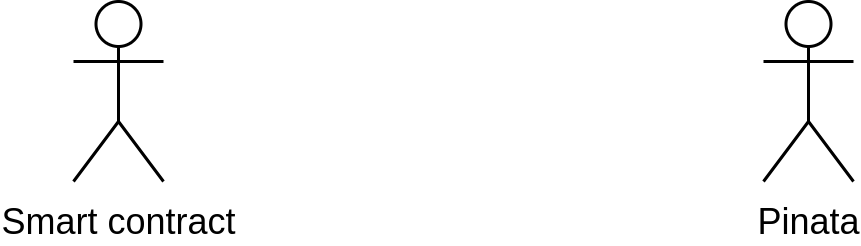
\includegraphics{capitolo3/casi-uso/attori-secondari.png}
  \caption{Attori secondari}
\end{figure}

\begin{itemize}
  \item \textbf{\textit{Smart contract}}: rappresenta lo \textit{smart contract} caricato in \textit{blockchain} con il quale comunicare;
  \item \textbf{Pinata}: rappresenta il servizio che permette di interagire con la rete IPFS.
\end{itemize}

\UC{Caricamento di un NFT in blockchain}
\label{UC:upload-new-nft}

Qualsiasi applicativo Java può caricare un nuovo NFT in \textit{blockchain}.

\begin{itemize}
  \item \UCPrimaryActors{applicativo Java};
  \item \UCSecondaryActors{\textit{smart contract} e Pinata};
  \item \UCPre{l'applicativo Java vuole creare un NFT da un'opera non ancora esistente};
  \item \UCPost{il NFT è stato creato e l'opera è stata caricata nella rete IPFS};
  \item \UCMain
  
  \begin{itemize}
    \item l'applicativo Java vuole creare un NFT a partire da un opera alla quale non è associato nessun altro NFT;
    \item l'opera viene caricata sulla rete IPFS tramite il servizio Pinata;
    \item viene invocato lo \textit{smart contract}, attraverso il \textit{wallet} del proprietario, e creato il NFT con le seguenti informazioni aggiuntive:
    \begin{itemize}
      \item il codice hash univoco che identifica il NFT;
      \item \textit{wallet} del creatore del NFT;
      \item l'identificativo con il quale il creatore del NFT viene riferito nel \textit{database} del \textit{back-end};
      \item il \textit{timestamp} dell'operazione.
    \end{itemize}
  \end{itemize}
  
  \item \UCExt
  \begin{enumerate}[label=\lett]
    \item l'applicativo Java vuole assegnare il NFT ad un \textit{wallet} che non è nel formato corretto:
    \begin{itemize}
      \item (UC\ref{UC:extension.wallet-not-correct}) - viene inviato il messaggio di \textit{wallet} non corretto;
      \item viene impedita la creazione del NFT.
    \end{itemize}

    \item l'applicativo Java vuole comunicare con lo \textit{smart contract} attraverso un \textit{wallet}, il quale non è il proprietario di quest'ultimo:
    \begin{itemize}
      \item (UC\ref{UC:extension.operation-not-allowed}) - viene inviato il messaggio di operazione non consentita;
      \item viene impedita la creazione del NFT.
    \end{itemize}

    \item l'applicativo Java vuole caricare un'opera dalla quale è già stato estratto il NFT:
    \begin{itemize}
      \item (UC\ref{UC:extension.nft-exists-yet}) - viene inviato il messaggio di NFT già esistente;
      \item viene impedita la creazione del NFT.
    \end{itemize}
  \end{enumerate}
\end{itemize}


\UC{Trasferimento della proprietà di un NFT}
\label{UC:transfer-nft}

L'applicativo Java può trasferire la proprietà di un NFT dal proprietario ad un acquirente.

\begin{itemize}
  \item \UCPrimaryActors{applicativo Java};
  \item \UCSecondaryActors{\textit{smart contract}};
  \item \UCPre{esiste il NFT che si vuole trasferire e l'acquirente è diverso dal proprietario};
  \item \UCPost{il NFT viene trasferito dal proprietario all'acquirente};
  
  \item \UCMain
  \begin{itemize}
    \item l'applicativo Java, attraverso il \textit{wallet} del proprietario dello \textit{smart contract}, comunica con quest'ultimo che è stato precedentemente caricato nella \textit{blockchain};
    \item invia i seguenti dati:
    \begin{itemize}
      \item l'identificativo con il quale è memorizzato il NFT all'interno dello \textit{smart contract};
      \item il \textit{wallet} del proprietario;
      \item l'identificativo con il quale il proprietario viene riferito nel \textit{database} del \textit{back-end};
      \item il \textit{wallet} dell'acquirente;
      \item l'identificativo con il quale l'acquirente viene riferito nel \textit{database} del \textit{back-end};
      \item il prezzo dell'acquisto, con relativa valuta;
      \item il \textit{timestamp} dell'operazione.
    \end{itemize}
    \item viene eseguito il trasferimento.
  \end{itemize}

  \item \UCExt
  \begin{enumerate}[label=\lett]
    \item l'applicativo Java vuole trasferire il NFT dal proprietario ad un acquirente, riferendosi ad uno di questi due attraverso un \textit{wallet} che non è nel formato corretto:
    \begin{itemize}
      \item (UC\ref{UC:extension.wallet-not-correct}) - viene inviato il messaggio di \textit{wallet} non corretto;
      \item viene impedito il trasferimento del NFT.
    \end{itemize}

    \item l'applicativo Java vuole comunicare con lo \textit{smart contract} attraverso un \textit{wallet}, il quale non è il proprietario di quest'ultimo:
    \begin{itemize}
      \item (UC\ref{UC:extension.operation-not-allowed}) - viene inviato il messaggio di operazione non consentita;
      \item viene impedito il trasferimento del NFT.
    \end{itemize}

    \item l'acquirente corrisponde al proprietario del NFT:
    \begin{itemize}
      \item viene inviato il messaggio di operazione non andata a buon fine, dato che l'acquirente non può essere lo stesso proprietario del NFT;
      \item viene impedito il trasferimento del NFT.
    \end{itemize}
  \end{enumerate}
\end{itemize}

\UC{Ottenimento di un NFT a partire dal suo id}
\label{UC:get-nft-by-id}

L'applicativo Java può ottenere le informazioni di un NFT a partire dall'identificativo con il quale è memorizzato.

\begin{itemize}
  \item \UCPrimaryActors{applicativo Java};
  \item \UCSecondaryActors{\textit{smart contract}};
  \item \UCPre{l'applicativo Java utilizza un id associato ad un NFT};
  \item \UCPost{l'applicativo Java ottiene le informazioni del NFT};
  \item \UCMain
  \begin{itemize}
    \item l'applicativo Java invoca lo \textit{smart contract} utilizzando un id associato ad un NFT;
    \item riceve le informazioni che sono state inserite durante la creazione.
  \end{itemize}

  \item \UCExt
  \begin{enumerate}[label=\lett]
    \item l'applicativo Java invia un id che non è associato ad alcun NFT:
    \begin{itemize}
      \item (UC\ref{UC:extension.nft-not-exists}) - viene inviato il messaggio di NFT non esistente.
    \end{itemize}
  \end{enumerate}
\end{itemize}

\UC{Ottenimento di un opera a partire dal suo hash}
\label{UC:get-nft-by-hash}

L'applicativo Java può ottenere le informazioni di un NFT a partire dal codice hash associato al NFT.

\begin{itemize}
  \item \UCPrimaryActors{applicativo Java};
  \item \UCSecondaryActors{\textit{smart contract}};
  \item \UCPre{l'applicativo Java utilizza un codice hash associato ad un NFT};
  \item \UCPost{l'applicativo Java ottiene le informazioni del NFT};
  
  \item \UCMain
  \begin{itemize}
    \item l'applicativo Java invoca lo \textit{smart contract} utilizzando il codice hash associato al NFT che vuole ottenere;
    \item riceve le informazioni che sono state inserite durante la creazione. 
  \end{itemize}
  
  \item \UCExt
  \begin{enumerate}[label=\lett]
    \item l'applicativo Java invia un hash che non è associato ad alcun NFT:
    \begin{itemize}
      \item (UC\ref{UC:extension.nft-not-exists}) - viene inviato il messaggio di NFT non esistente.
    \end{itemize}
  \end{enumerate}
\end{itemize}

\UC{Ottenimento della storia delle transazioni di un NFT}
\label{UC:get-transaction-history}

L'applicativo Java può ottenere la storia delle transazioni di un NFT a partire dal id con il quale è memorizzato dentro lo \textit{smart contract}.

\begin{itemize}
  \item \UCPrimaryActors{applicativo Java};
  \item \UCSecondaryActors{\textit{smart contract}};
  \item \UCPre{l'applicativo Java utilizza un id associato ad un NFT};
  \item \UCPost{l'applicativo Java ottiene la storia delle transazioni di un NFT};

  \item \UCMain
  \begin{itemize}
    \item l'applicativo Java invoca lo \textit{smart contract} utilizzando un id associato ad un NFT;
    \item riceve la storia delle transazioni con tutte le informazioni che vengono inserite ad ogni trasferimento di proprietà.
  \end{itemize}
  
  \item \UCExt
  \begin{enumerate}[label=\lett]
    \item l'applicativo Java invia un id che non è associato ad alcun NFT:
    \begin{itemize}
      \item (UC\ref{UC:extension.nft-not-exists}) - viene inviato il messaggio di NFT non esistente.
    \end{itemize}
  \end{enumerate}
\end{itemize}

\UC{Messaggio di wallet non corretto}
\label{UC:extension.wallet-not-correct}

Nel caso in cui il \textit{wallet} inviato allo \textit{smart contract} non sia nel formato corretto, verrà inviato un messaggio di errore che lo segnalerà.

\begin{itemize}
  \item \UCPrimaryActors{applicativo Java};
  \item \UCSecondaryActors{\textit{smart contract}};
  \item \UCPre{il formato del \textit{wallet} non è nel formato corretto};
  \item \UCPost{viene inviato il messaggio di \textit{wallet} non corretto};
  
  \item \UCMain
  \begin{itemize}
    \item l'applicativo Java invia un \textit{wallet} allo \textit{smart contract} che non è nel formato corretto;
    \item viene inviato il messaggio di \textit{wallet} non corretto.
  \end{itemize}
\end{itemize}

\UC{Messaggio di operazione non consentita}
\label{UC:extension.operation-not-allowed}

Nel caso in cui lo \textit{smart contract} non venga invocato dal suo proprietario, verrà inviato il messaggio di operazione non consentita.

\begin{itemize}
  \item \UCPrimaryActors{applicativo Java};
  \item \UCSecondaryActors{\textit{smart contract}};
  \item \UCPre{lo \textit{smart contract} non viene invocato dal suo proprietario};
  \item \UCPost{viene inviato il messaggio di operazione non consentita};
  
  \item \UCMain
  \begin{itemize}
    \item l'applicativo Java non viene invocato dal suo proprietario;
    \item viene inviato il messaggio di operazione non consentita. 
  \end{itemize}
\end{itemize}

\UC{Messaggio di NFT già esistente}
\label{UC:extension.nft-exists-yet}

Nel caso in cui si cerchi di caricare un NFT già esistente, verrà inviato un messaggio di errore opportuno che lo segnalerà.

\begin{itemize}
  \item \UCPrimaryActors{applicativo Java};
  \item \UCSecondaryActors{\textit{smart contract}};
  \item \UCPre{l'applicativo Java carica un NFT già esistente};
  \item \UCPost{viene inviato il messaggio di NFT già esistente};
  
  \item \UCMain
  \begin{itemize}
    \item l'applicativo Java carica un NFT già esistente;
    \item viene inviato il messaggio di NFT già esistente.
  \end{itemize}
\end{itemize}

\UC{Messaggio di NFT non esistente}
\label{UC:extension.nft-not-exists}

Nel caso in cui il NFT di cui si ha bisogno non esista, verrà inviato un messaggio opportuno che lo segnalerà.

\begin{itemize}
  \item \UCPrimaryActors{applicativo Java};
  \item \UCSecondaryActors{\textit{smart contract}};
  \item \UCPre{il NFT che si sta cercando non esiste};
  \item \UCPost{viene inviato un messaggio di errore che segnala la non esistenza del NFT};
  
  \item \UCMain
  \begin{itemize}
    \item l'applicativo Java ha bisogno di un NFT non esistente;
    \item viene inviato il messaggio di NFT non esistente.
  \end{itemize}
\end{itemize}

\subsection{Requisiti}
I requisiti individuati per il progetto sono riportati di seguito, insieme ad una descrizione che lo descrive e la fonte da cui deriva. \\

\noindent La classificazione dei requisiti ha seguito la seguente convenzione:
\begin{center}
  R(Tipo)(Importanza)[0-9]+
\end{center}
dove:
\begin{itemize}
  \item il tipo può essere assumere le seguenti categorie:
  \begin{itemize}
    \item \textbf{F}: rappresenta un requisito funzionale;
    \item \textbf{Q}: rappresenta un requisito di qualità;
    \item \textbf{V}: rappresenta un requisito di vincolo.
  \end{itemize}

  \item l'Importanza può assumere i seguenti valori:
  \begin{itemize}
    \item \textbf{O}: rappresenta un requisito obbligatorio;
    \item \textbf{D}: rappresenta un requisito desiderabile;
    \item \textbf{F}: rappresenta un requisito facoltativo.
  \end{itemize}
\end{itemize}

\noindent Per quanto riguarda la fonte da cui deriva un requisito, può essere di tre tipi:
\begin{itemize}
  \item \textbf{Caso d'uso}: il requisito è derivato in seguito all'analisi di un caso d'uso;
  \item \textbf{Interna}: il requisito è derivato da una decisione mia, ovviamente approvata e discussa con il mio \textit{tutor} aziendale, Fabio Pallaro;
  \item \textbf{Esterna}: il requisito è derivato da una decisione presa dal proponente. 
\end{itemize}

\subsubsection{Requisiti funzionali}
\begin{longtabu}{|X[0.8,c]|X[3,c]|X[0.5,c]|}
  \hline 

  \textbf{Codice requisito} & \textbf{Descrizione} & \textbf{Fonte} \\ 

  \hline

  \rfun{O}{} & L'applicativo Java può caricare un nuovo NFT. & UC\ref{UC:upload-new-nft} \\
  
  \hline

  \rfun{O}{} & L'applicativo Java può trasferire la proprietà di un NFT dal proprietario ad un acquirente. & UC\ref{UC:transfer-nft} \\ 
  
  \hline

  \rfun{O}{} & L'applicativo Java può ottenere le informazioni di un NFT a partire dall'id con il quale è memorizzato all'interno dello \textit{smart contract}. & UC\ref{UC:get-nft-by-id} \\ 
  
  \hline

  \rfun{O}{} & L'applicativo Java può ottenere le informazioni di un NFT a partire dal codice hash al quale è associato. & UC\ref{UC:get-nft-by-hash} \\ 
  
  \hline

  \rfun{O}{} & L'applicativo Java può ottenere la storia delle transazioni di un NFT. & UC\ref{UC:get-transaction-history} \\ 
  
  \hline

  \caption{Requisiti funzionali}
\end{longtabu}

\subsubsection{Requisiti di qualità}
\begin{longtabu}{|X[0.8,c]|X[3,c]|X[0.5,c]|}

  \hline 

  \textbf{Codice requisito} & \textbf{Descrizione} & \textbf{Fonte} \\ 

  \hline

  \rqua{O} & Tutto il \textit{software} prodotto deve essere rilasciato sotto licenza MIT & Interna \\
  
  \hline

  \rqua{O} & Tutto il \textit{software} prodotto dovrà superare la soglia ottimale del 90.0\% di \textit{statements coverage} & Interna \\
  
  \hline

  \rqua{O} & Tutto il \textit{software} prodotto dovrà superare la soglia ottimale del 90.0\% di \textit{branches coverage} & Interna \\
  
  \hline

  \rqua{O} & Tutto il \textit{software} prodotto dovrà superare la soglia ottimale del 90.0\% di \textit{functions coverage} & Interna \\
  
  \hline

  \rqua{O} & Tutto il \textit{software} prodotto dovrà superare la soglia ottimale del 90.0\% di \textit{lines coverage} & Interna \\
  
  \hline

  \caption{Requisiti di qualità}
\end{longtabu}

\subsubsection{Requisiti di vincolo}
\begin{longtabu}{|X[0.8,c]|X[3,c]|X[0.5,c]|}

  \hline 

  \textbf{Codice requisito} & \textbf{Descrizione} & \textbf{Fonte} \\

  \hline

  \rvin{O} & Il linguaggio di programmazione per la scrittura dello \textit{smart contract} in Ethereum dovrà essere Solidity & Esterna \\ 
  
  \hline

  \rvin{O} & La libreria deve funzionare correttamente con JavaSE 15 in poi & Esterna \\
  
  \hline

  \rvin{O} & Si dovrà utilizzare il protocollo IPFS per il salvataggio delle opere & Interna \\
  
  \hline

  \caption{Requisiti di vincolo}
\end{longtabu}
